\subsection{Gráfico}

\begin{example}
    Seja $f: \R \to \R_+^*$ uma função exponencial tal que $f(x) =
a^x$. Na Imagem~\ref{img:graficos-exponencial}, são mostrados os gráficos
nos casos de $a > 1$ e $0 < a < 1$.
%
\begin{figure}[H]
    \centering
    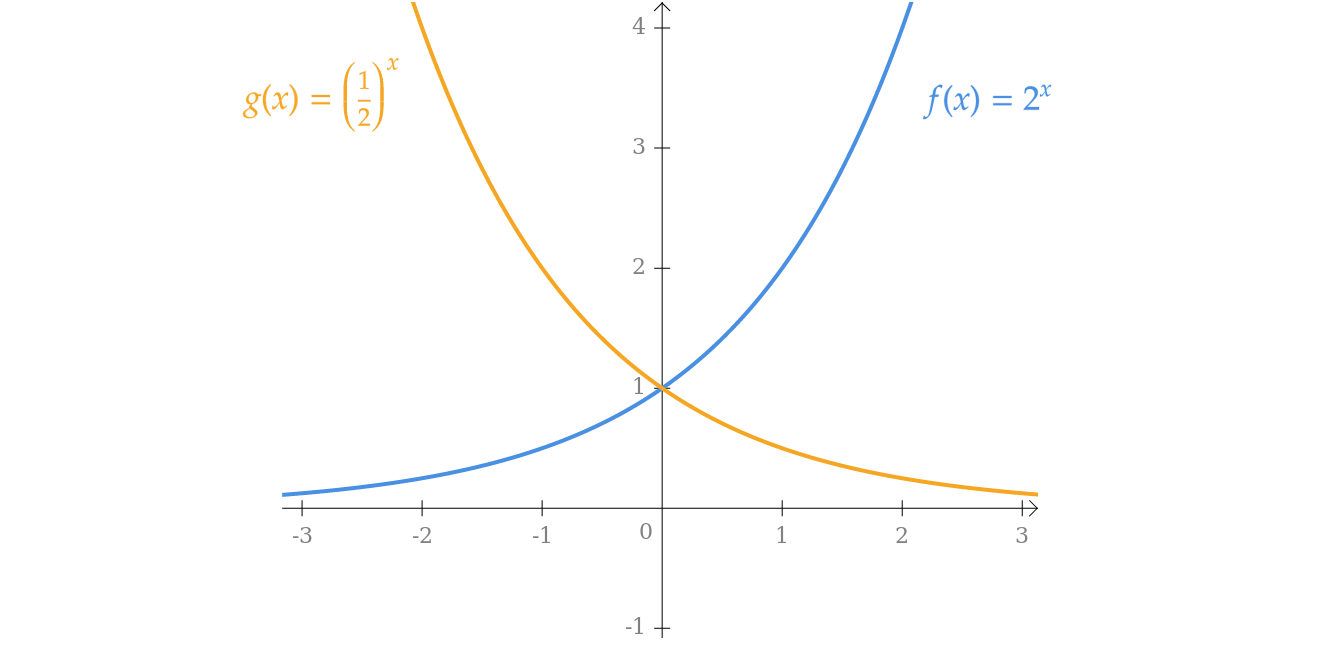
\includegraphics[scale=0.30]{\imgdirfromsection/grafico-exponencial.png}
    \caption{Gráficos da função $f$ nos casos $0<a<1$ e $a>1$.}
    \label{img:graficos-exponencial}
\end{figure}
%
O gráfico de $f$ nunca toca o eixo $x$, mas fica tão próximo quanto
queiramos. Isso equivale dizer que a reta $y=0$ é \textdef{assíntota} do
gráfico de $f$.
\end{example}

\begin{remark}
    Quando as bases de duas funções exponenciais são uma o inverso multiplicativo da outra, o gráfico de uma 
    das funções consiste em uma reflexão do da outra. Em outras palavras, se $f:\reais \to \preais$
    tal que $f(x) = a^x $ para certo $a > 0$, então a função $g:\reais \to \preais$ com regra 
    $g(x) = \frac 1 a$ é tal que:
    %
    \[
        g(x) = \frac 1 a = a^{-1} = f(-1),    
    \]
    e, conforme visto na Seção \ref{sec:dilatacao-e-reflexao}, o gráfico de $g$ é obtível a partir do $f$ refletindo-o em relação ao eixo
    $y$. Ademais, note que, como $a > 0$ e $a \ne 1$, temos que:
    %
    $$a > 1 \iff 0 < \frac{1}{a} < 1.$$
\end{remark}

\begin{example}
    O crescimento exponencial supera o de qualquer polinômio. Ao compararmos, por exemplo, as funções $f(x) = 2^x$ e $p(x)=x^{10}$, temos que:
    \begin{align*}
        0<x<1{,}077 & \implies  2^x > x^{10} \\
        1{,}077 < x < 58{,}77 & \implies  x^{10} > 2^x \\
        x>58{,}77 & \implies  2^x > x^{10}
    \end{align*}
\end{example}

\begin{onlineact}
    \khan{https://pt.khanacademy.org/math/algebra/introduction-to-exponential-functions/exponential-expressions-alg1/e/exponential-expressions-word-problems-algebraic}
    {Problemas (Algébricos) de Expressões Exponenciais}
\end{onlineact}

\begin{onlineact}
    \khan{https://pt.khanacademy.org/math/algebra/introduction-to-exponential-functions/exponential-decay-alg1/e/graphs-of-basic-exponential-functions}
    {Representação Gráfica de Crescimento e Decaimento Exponencial}
\end{onlineact}

\begin{onlineact}
    \khan{https://pt.khanacademy.org/math/algebra2/exponential-and-logarithmic-functions/graphs-of-exponential-functions/e/graphs-of-exponential-functions}
    {Gráficos de Funções Exponenciais}
\end{onlineact}